\begin{titlepage}
%
\begin{minipage}[t]{0.45\textwidth}
\begin{flushleft} \large
\includegraphics[width=0.8\textwidth]{./pictures/bci_logo}~\\[1cm]
\end{flushleft}
\end{minipage}
%
\hfill
%
\begin{minipage}[t]{0.45\textwidth}
\begin{flushright} \large 
\includegraphics[width=0.8\textwidth]{./pictures/bci_logo}~\\[1cm]
\end{flushright}
\end{minipage}
%
\noindent\makebox[\linewidth]{\textcolor{black!30!white}{\rule{0.98\textwidth}{1pt}}}
\centerline{Chair of Reaction Engineering}\\
\centerline{Prof. Dr. David W. Agar}\\
%
\begin{center}
%
\begin{LARGE}    
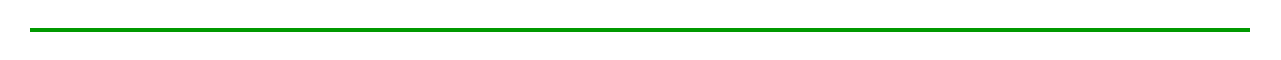
\begin{tikzpicture}
\draw[green!60!black, ultra thick](0,0) -- (15.5,0);
\end{tikzpicture} 
\\[0.5 cm]
\textbf{Optimisation and Implementation of a non-invasive measurement technique to monitor liquid-liquid slug flow in micro-channels}
\\[0.5 cm]
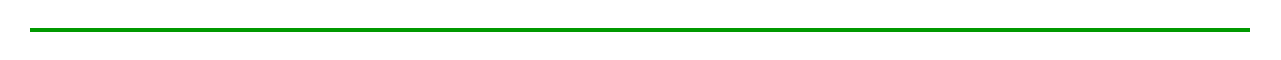
\begin{tikzpicture}
\draw[green!60!black, ultra thick](0,0) -- (15.5,0);
\end{tikzpicture} 
\end{LARGE}%
\\[1cm]
\centerline{\textbf{\Large Master Thesis}}
%
\noindent\parbox[c][2cm][c]{0.7\textwidth}{\centering \emph{\normalsize submitted in the fulfilment of requirements for the degree of Master of Science in Chemical Engineering}}\\[1.75cm]
%
\textbf{Author:}\\ Shoneil Oswal\\[0.5cm]
\textbf{Supervising professors:}\\ Prof. Dr. David W. Agar\\Prof. Dr.-Ing. Sebastian Engell\\[0.5cm]
\textbf{Supervisor:}\\ M. Sc. Linda Arsenjuk\\[1.75cm]
Dortmund, \today\\
%
\vspace*{-1cm}
%\fancyfoot[R]{\vspace{-.1cm}\hspace{1cm}\includegraphics[width=3cm]{./pictures/bci_logo}}
%
%\fancyfoot[C]{\scriptsize Department of Biochemical and Chemical Engineering\\Technische Universit�t Dortmund}
%
%\fancyfoot[L]{\vspace{-.25cm}
\includegraphics[width=3cm]{./pictures/ad_logo}}
%
\end{center}
\end{titlepage}
